\documentclass[a4paper,11pt]{jsarticle}

% 数式
\usepackage{amsmath,amsfonts}
\usepackage[dvipdfmx]{graphicx}
\usepackage{bm}
\usepackage{listings, jlisting}
% 画像
\usepackage[dvipdfmx]{graphicx}

\lstset{language=,%
        basicstyle=ootnotesize,%
        commentstyle=	extit,%
        classoffset=1,%
        keywordstyle=fseries,%
        frame=tRBl,framesep=5pt,%
        showstringspaces=false,%
        breaklines=true%
        }%

\begin{document}

\title{JPHACKSにおけるアイトラッキング技術の開発}
\author{ずっとエイリアンでいいのに}
\date{\today}
\maketitle

\section{はじめに}
JPHACKS1日目, 我々はある決断をした.

「漫画のコマを見ると音がなるサービス」この開発には, 正確なアイトラッキング技術が必要であった.
我々は当時, アイトラッキングの技術は発展しているしこの部分は問題ないだろうと楽観視していた.

しかし, 現実はそんなに甘くなかった.
既存のWebカメラを用いたアイトラッキング技術では, 求める精度には及ばなかった.
我々は決断を迫られた.
アイデアを変えるか, それともこのまま続けるか.

確かに, 既存のアイトラッキングの精度はそれほど高くはない.
しかしこれはハッカソンだ, そこまで要求はされないだろう.
その考えが頭によぎった.
そう, これが2日間のハッカソンならそれで良かったのだ.

我々には1週間の時間が与えられた.
既存の技術を使うなら2日あれば終わってしまう.
我々にはそれ以上が求められた...

よかろう, それなら, アイトラッキングを自作してやるよ.

\section{先行研究}
アイトラッキングについての知識は一切無かったため, 既存技術の調査を行った. 以下はその代表的なものである.
\subsection{角膜反射法}
非常に精度の高いアイトラッキングシステムとして, 角膜反射法を用いたものがある.
これはカメラ位置から赤外線を飛ばし黒目に投影された点と黒目の位置 (正確には瞳孔とプルキニエ像)の
位置関係によって視線を推定するという技術である. (図 \ref{fig:kakumaku})

\begin{figure}
  \begin{center}
    \includegraphics[width=7.0cm]{kakumaku.png}
    \caption{角膜反射法}
    \label{fig:kakumaku}
  \end{center}
\end{figure}

精度が高く多くのアイトラッキングシステムに組み込まれているが, カメラ位置から赤外線を発する必要がある為, 通常のウェブカメラではなく専用のセンサーが必要となる.
本開発では, 汎用的なアイトラッキングシステムとしてPC付属のウェブカメラを利用したい. その為, 角膜反射法を利用する事ができない
事になる.

\subsection{WebGazer}
ウェブカメラを用いたアイトラッキングシステムはいくつか存在する. その内の一つがWebGazerである. 
WebGazerはオープンソースのプロジェクトでブラウザ上で実行可能なデモも公開されている. 

他にもウェブカメラを用いたアイトラッキングシステムは存在するが, ブラウザ上で動作する物は少ない. 
また, ブラウザ上で動作してもWebGazerと精度は似ている印象を受けた. WebGazerは論文も公開しており, 詳細な実験結果等を確認可能である. \cite{webgazer}

WebGazerのアイトラッキング手法を簡潔にまとめると, 下記のようになる.
\begin{enumerate}
  \item カメラ画像から目の画像を抽出
  \item 抽出した画像を前処理
  \item 目の画像からすくリー座標を予測
\end{enumerate}

これらは次の章で詳しく説明を加える.

\section{独自実装}
既存システムでは私たちの求める精度は得られなかった. 
そこで我々はWebGazerをベースに, より精度の高いアイトラッキングを開発することにした.

コードの拡張性を増やす既存のライブラリを用いず, まずはWebGazerの必要部分のみを簡潔に再現することにした.
いわば車輪の再発明であるが, WebGazerのコードは数々の実験によって膨れ上がっており, またコードのミスも散見された. 
従って情報を絞り拡張性を高めるこの作業には大きな意味があったといえる.

以下はWebGazerの論文を読み, それを元に実際に我々が実装した手法である.

\subsection{Facemeshによる目の画像抽出}
Facemeshと呼ばれる顔認識を行いキーポイントを抽出する事ができるライブラリを利用し, ウェブカメラの情報から目の位置を推定, 画像を切り抜いた. 
Facemeshはブラウザ上で動作する程軽いため, サーバーとの不要な通信も避ける事ができた.

\subsection{目の画像の前処理}
\subsubsection{解像度}
Webブラウザ上で動作させる為, 重い処理はなるべく避けたい. 
画像の解像度は計算量に多きな影響を与えるため, WebGazerでは片目を縦6×横10に分割しており, 我々もそれに習う事としに習う事とした.

\subsubsection{グレースケール化}
目の色の情報は視線推定には関係が薄い. 
計算量の削減のためにグレースケールに変換する.

\subsubsection{ヒストグラム標準化}
グレースケールでも画像によって光の加減が違う. 
暗い画像や明るい画像が同等に扱われてしまうと, 問題が生じる可能性が高い.
その為, 相対的な色の情報として捉えられるようにヒストグラム標準化というものを行う.

\subsection{目の画像からスクリーン座標を推定}
目の画像は前処理を経て縦6×横10次元の画像が両目で, 合計120次元の情報となる.
これを2次元のスクリーン座標に変換する必要がある.
WebGazerではこれを, リッジ回帰で実現していた.

しかし, tensorflow.jsは逆関数やLU分解が実装されておらず, リッジ回帰は非常に導入コストが高い.
そこで我々はこの部分においてはtensorflow.jsを用いた学習によって, リッジ回帰と同等の内容を実現した.

\subsection{キャリブレーション}
上記内容を事前に得たラベル付きデータからリッジ回帰の係数を計算する.
大抵の場合, これはブラウザで各個人に合わせてサービス利用直前に行われる.

例えば画面に表示された点を目で追う事で点の位置を正解データ, その時の目の画像を入力とする.
この作業はキャリブレーションと呼ばれる.

\begin{figure}
  \begin{center}
    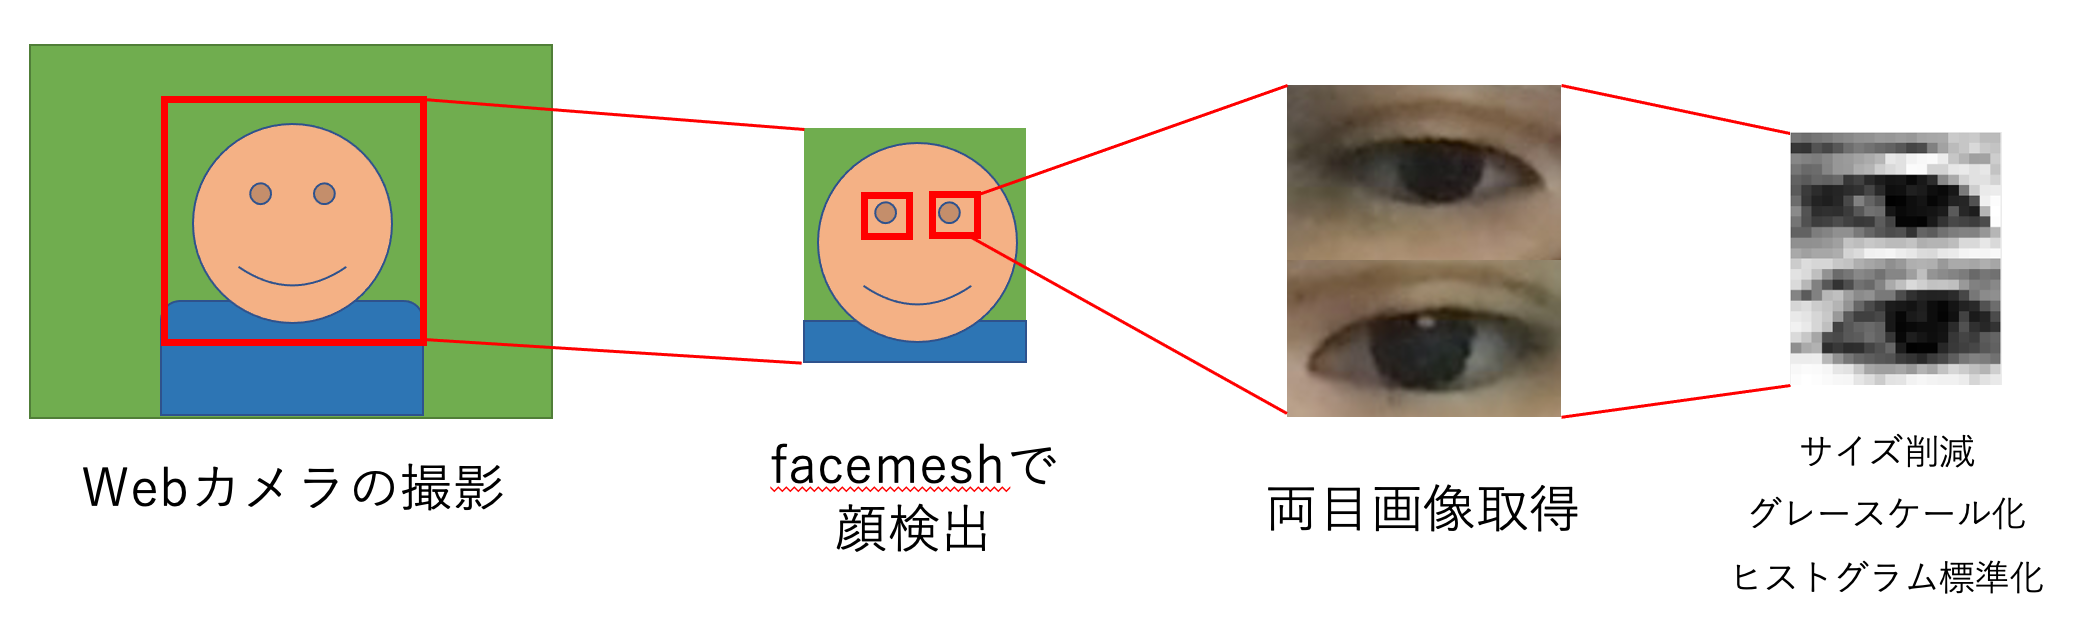
\includegraphics[width=7.0cm]{getEyes.png}
    \caption{}
    \label{fig:kakumaku}
  \end{center}
\end{figure}

\section{提案手法}
我々はここでようやくスタートラインに立った.
WebGazerの精度を超えるべく, 我々の考えた新しい手法を提案する. 
(もしかしたら既に行われている手法もあるかもしれないが, 少なくともWebGazerにはない我々が考えた新しい手法である.)

\subsection{CNNの利用による解像度の向上}
\subsubsection{概要}
WebGazerでは, 縦6×横10次元の目の画像から2次元の座標を予測していた. これは明らかに解像度が低いと言える.

WebGazerでは, 120次元の画像データを2次元に変換するのにリッジ回帰を用いていた.
しかしリッジ回帰はLU分解を必要とし, これが $o(n^3):$ であるために画像の次元を増やせば爆発的に計算量が増えた.
この為, 目の画像の解像度をあげられなかった.

我々は, この問題を解決するためにCNNを導入することにした.
CNNは並列処理かつオンラインで学習をできるため, 画像の次元数が増えても処理時間の増え方はそれほど大きくはない.
これによって, 画像の解像度をあげる事が可能となる.
画像の解像度が上がればより細かい目の動きも反映ができ, 精度が上がるのではないかと考えた.

\subsubsection{実験方法}
ブラウザ上でCNNを使う為にtensorflow.jsを利用して, WebGLをバックエンドに使用した.
これによって, サーバーとの通信を必要とせずフロントエンドのみで学習を可能とした.

この条件で画像の解像度をあげて, 精度の変化を確認した.

\subsubsection{実験結果}
画像解像度を2倍, 4倍にあげたところ, 学習時間は大きくは変わらなかった.
精度については, 少なくとも悪くなってはいないが目立った向上もないように思えた.

定量的な評価については, 例えばある点を見て予測点との距離が閾値未満なら正, 閾値以上なら負をする事が出来ず, 申し訳ない.

\begin{figure}
  \begin{center}
    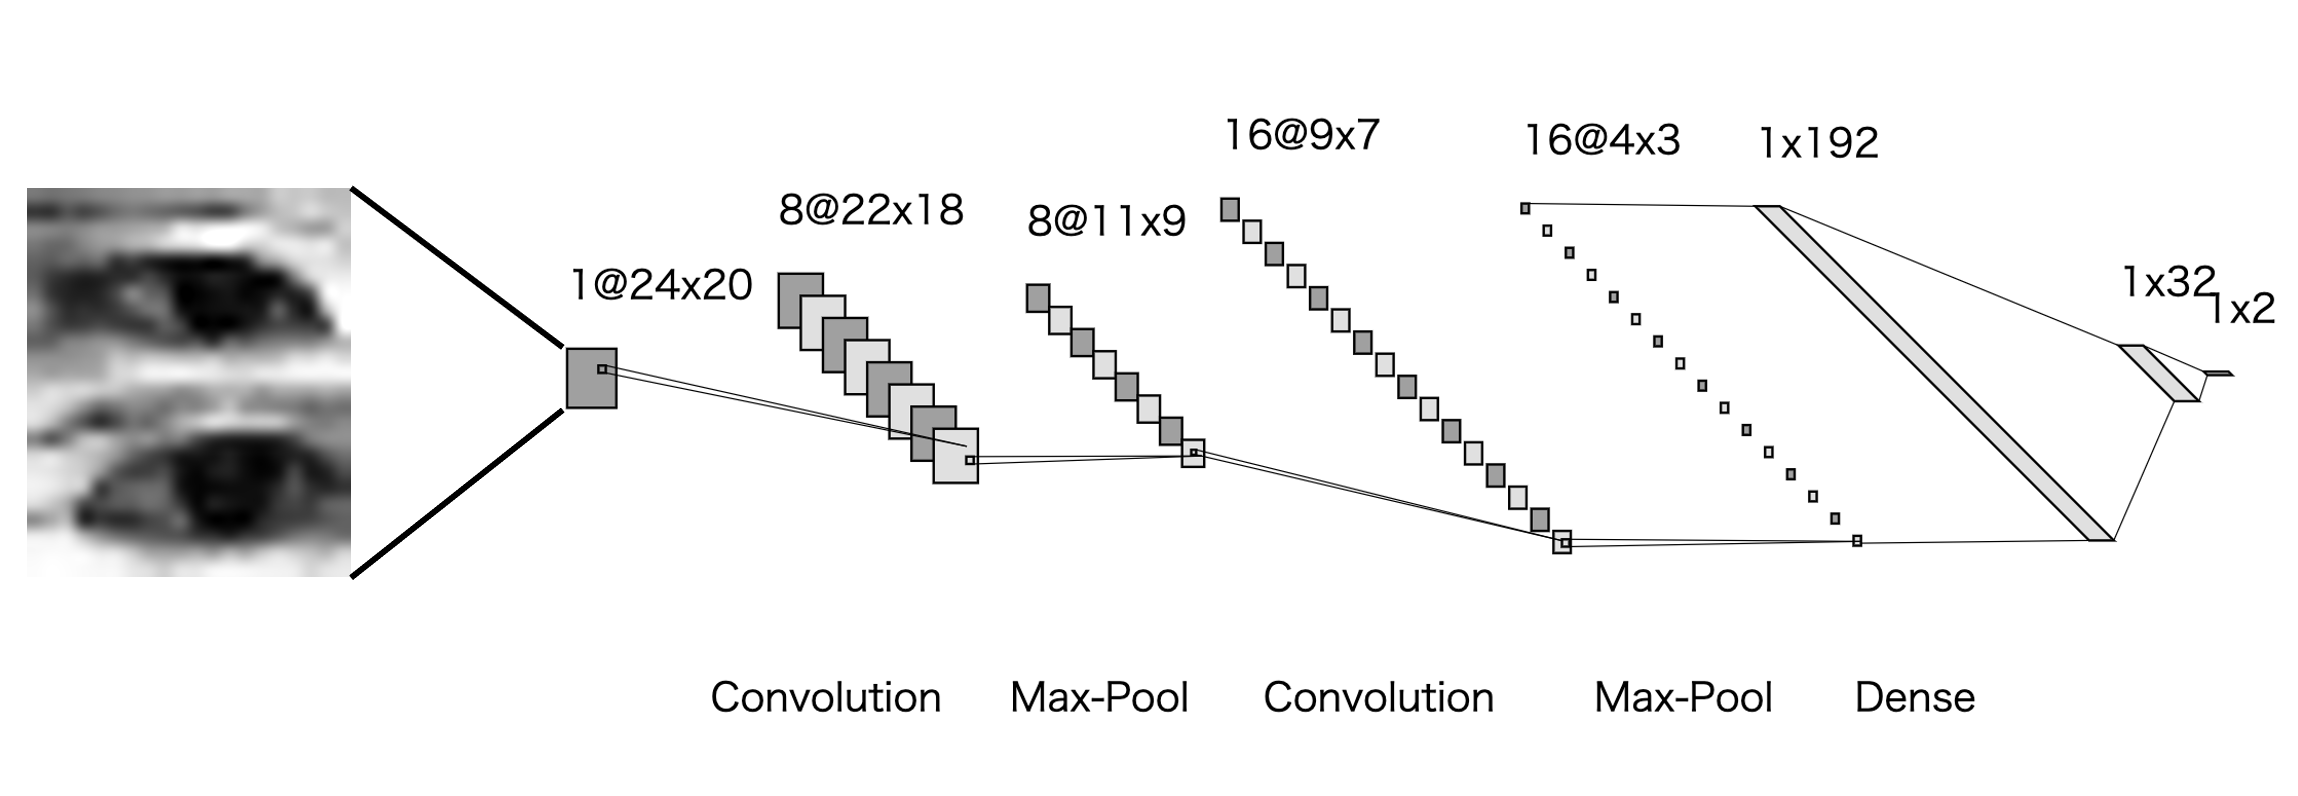
\includegraphics[width=7.0cm]{cnn.png}
    \caption{}
    \label{fig:kakumaku}
  \end{center}
\end{figure}

\subsection{キャリブレーション方法の変更}
\subsubsection{概要}
WebGazerではマウスをクリックした位置をキャリブレーション用のデータとしていたが, これは手間であり, また人によって差が生じる.
従って, 基本的に自動で動く点を目で追いかける事でキャリブレーションを行うことにした. 
この点の動かし方についてもいくつかの手法を試した.

\subsubsection{実験方法}
下記4つの手法について実装し, 精度の検証を行った.
\begin{enumerate}
  \item{左上から右下に横方向に走査} ブラウザ左上から, 右に向かって点を動かし右端に着いたら少し下に動き左に移動. これを繰り返す.
  \item{右下から左上に横方向に走査} ブラウザ右下から, 左に向かって点を動かし左端に着いたら少し上に動き右に移動. これを繰り返す.
  \item{ランダムに走査} ランダムな位置に点を表示
  \item{全体的に走査} 左上, 右下, 右上, 左下, 中上, 中下, 左中, 右中の順に走査
\end{enumerate}

\subsubsection{実験結果}
1の手法を行ったところ,  予測した視線位置は上に偏った. 
また, 左右の目の移動に関しては精度が高く敏感に反応したが, 上下の目の移動については反応が鈍かった.
特に画面下部を見るのはかなり厳しかった.

2の手法を行ったところ, 1とは逆の結果となった. 視線は下部に集中し, 画面上部をみるのは厳しかった.
左右の移動に敏感で, 上下の移動に鈍いのは同様であった.

3の手法を行ったところ, 1, 2とは違い上下の移動に関する制限は無いように感じた.
しかし, 視線が画面中央にやや寄っており, 画面端を見るのが難しかった.

4の手法を行ったところ, 上下の移動に関する制限はなくかなり広範囲に視線移動ができた.
画面端を見る事が可能になったが, 代わりに画面中央付近の精度はやや下がった.

上記結果から, 我々は画面全体の移動を重視して4の手法を用いることにした.

\subsubsection{考察}
1, 2の手法について, 画面の上下の移動が制限されたのは目の移動だけでなく首の移動による視線の移動を行ったからではないかと考える.
始めに上部を重点的に走査すると, 楽に見る為に顔をやや上に傾けるのではないだろうか. 
顔の角度が変わると, 視線の推定は大きくずれる. 

3の手法については, ランダムな値である為に画面端の点を見る確率が低くなるため, 中央によったと考えられる.

逆に4の手法については, 画面中央の点を学習していないために画面全体が見やすくなったと思われる.

\subsection{補正}
\subsubsection{概要}
上述した手法で学習した機械学習モデルの予測結果に, さらにルールベースの修正や幾何的な計算を加えることでより精度の向上をめざす.
\subsubsection{顔の向きをもとに補正}
顔が右を向いているときには右方向に補正, 左なら左に補正を行う.
顔の向きに関する情報はFacemeshの頭頂部と顎先, 両目のキーポイントから算出した.
これは, キャリブレーション時には画面に対して首の傾きが0であるという前提で補正をした.
従って, 補正値が必要以上に働きすぎてしまう問題が生じた. 
残念ながらハッカソン期間内ではこの問題の解決にはいたらず, サービスへ組み込むのは見送ることにした.

\subsubsection{顔の位置をもとに補正}
顔の位置が右にある時には, 右方向に補正する.
これも学習時の位置が正面であり, 画面との距離が一定の距離であることが前提となっており, これが原因で補正が必要以上にかかったり, 弱かったりした.

\subsubsection{顔の大きさをもとに補正}
画面との距離によって, 目線位置は補正されるべきであると考えられる.
画面との距離はカメラの中の顔の比率によって測れるだろうと考えられる.

\subsubsection{中央値を利用}
視線推定にはノイズが多い. 
このノイズを吸収する手法として, 平均値などが考えられるが, 今回は中央値を用いることにした.
これは, 平均値は外れ値に引っ張られる可能性がある為である.

算出の際に考慮する過去のデータ数は安定性とリアルタイム性がトレードオフの関係にある.
今回は20回程度の情報を元に算出するのが良さそうであった.

\subsubsection{カルマンフィルター}
ひとつ前の予測値および, 今回の観測値を元に真の値を算出する手法としてカルマンフィルターがある.
これはノイズを吸収する方法として知られており, 適用できそうに見えた.

しかし目線は等速でも, 等加速度でも動くとは思えない為, シンプルな実装を行うと逆に精度が下がるという結果にいたる.

\subsubsection{考察}
この機能の一部は機械学習のインプットとして与え学習する事も出来, 実際に我々はそれを試した.
しかし学習の際には顔の向きや位置を動かさないため, この情報はむしろノイズとなり精度が下がった.
そのためあえて補正という形をとった. しかし, これも学習時の状態に依存するためになかなか難しいという印象であった.

\section{おわりに}
結果として我々は, 既存のライブラリであるWebGazerの精度を超えることができた.
たった一週間で0からアイトラッキングを学びそれを超える技術を作ろうという無謀にも見える挑戦を見事にやり遂げた, クレイジーなメンバーに敬意を表したい.

\begin{thebibliography}{}
  \bibitem{kakumaku} 目は口ほどに物を言う。「アイトラッキングの原理とアウトプット例」 https://techblog.nhn-techorus.com/archives/3435
  \bibitem{webgazer} WebGazer: Scalable Webcam Eye Tracking Using User Interactions http://cs.brown.edu/people/apapouts/papers/ijcai2016webgazer.pdf
\end{thebibliography}

\end{document}